\section{mo\-Fit\-Sol\-Continue$<$ EOT $>$ Class Template Reference}
\label{classmo_fit_sol_continue}\index{moFitSolContinue@{moFitSolContinue}}
One possible stop criterion for a solution-based heuristic.  


{\tt \#include $<$mo\-Fit\-Sol\-Continue.h$>$}

Inheritance diagram for mo\-Fit\-Sol\-Continue$<$ EOT $>$::\begin{figure}[H]
\begin{center}
\leavevmode
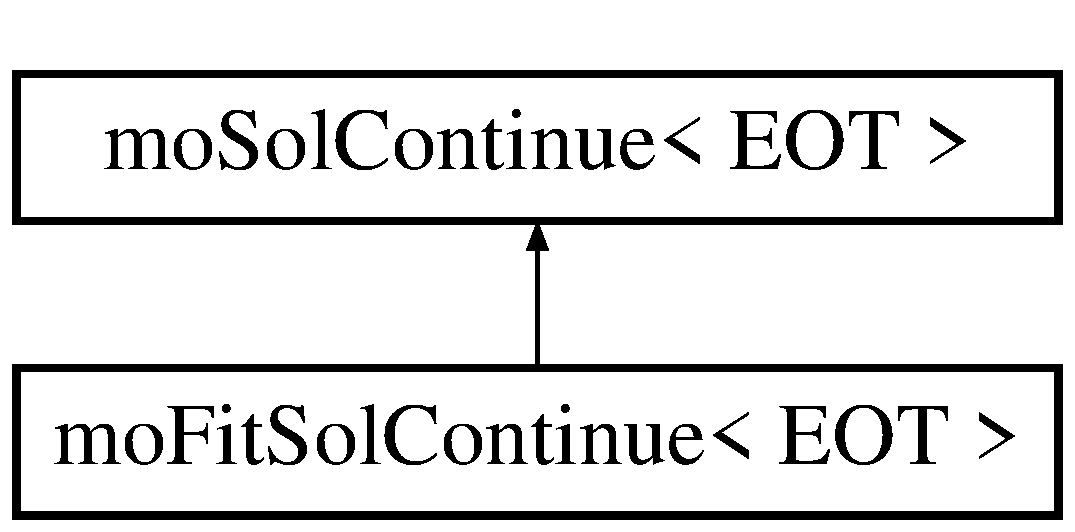
\includegraphics[height=4cm]{classmo_fit_sol_continue}
\end{center}
\end{figure}
\subsection*{Public Types}
\begin{CompactItemize}
\item 
typedef EOT::Fitness {\bf Fitness}\label{classmo_fit_sol_continue_w0}

\begin{CompactList}\small\item\em Alias for the fitness. \item\end{CompactList}\end{CompactItemize}
\subsection*{Public Member Functions}
\begin{CompactItemize}
\item 
{\bf mo\-Fit\-Sol\-Continue} ({\bf Fitness} \_\-fitness)
\begin{CompactList}\small\item\em Basic constructor. \item\end{CompactList}\item 
bool {\bf operator()} (const EOT \&\_\-solution)
\begin{CompactList}\small\item\em Function that activates the stopping criterion. \item\end{CompactList}\item 
void {\bf init} ()
\begin{CompactList}\small\item\em Procedure which allows to initialise all the stuff needed. \item\end{CompactList}\end{CompactItemize}
\subsection*{Private Attributes}
\begin{CompactItemize}
\item 
{\bf Fitness} {\bf fitness}\label{classmo_fit_sol_continue_r0}

\begin{CompactList}\small\item\em Fitness target. \item\end{CompactList}\end{CompactItemize}


\subsection{Detailed Description}
\subsubsection*{template$<$class EOT$>$ class mo\-Fit\-Sol\-Continue$<$ EOT $>$}

One possible stop criterion for a solution-based heuristic. 

The stop criterion corresponds to a fitness threshold gained. 



Definition at line 46 of file mo\-Fit\-Sol\-Continue.h.

\subsection{Constructor \& Destructor Documentation}
\index{moFitSolContinue@{mo\-Fit\-Sol\-Continue}!moFitSolContinue@{moFitSolContinue}}
\index{moFitSolContinue@{moFitSolContinue}!moFitSolContinue@{mo\-Fit\-Sol\-Continue}}
\subsubsection{\setlength{\rightskip}{0pt plus 5cm}template$<$class EOT$>$ {\bf mo\-Fit\-Sol\-Continue}$<$ EOT $>$::{\bf mo\-Fit\-Sol\-Continue} ({\bf Fitness} {\em \_\-fitness})\hspace{0.3cm}{\tt  [inline]}}\label{classmo_fit_sol_continue_a0}


Basic constructor. 

\begin{Desc}
\item[Parameters:]
\begin{description}
\item[{\em \_\-fitness}]The fitness to reach. \end{description}
\end{Desc}


Definition at line 57 of file mo\-Fit\-Sol\-Continue.h.

References mo\-Fit\-Sol\-Continue$<$ EOT $>$::fitness.

\subsection{Member Function Documentation}
\index{moFitSolContinue@{mo\-Fit\-Sol\-Continue}!operator()@{operator()}}
\index{operator()@{operator()}!moFitSolContinue@{mo\-Fit\-Sol\-Continue}}
\subsubsection{\setlength{\rightskip}{0pt plus 5cm}template$<$class EOT$>$ bool {\bf mo\-Fit\-Sol\-Continue}$<$ EOT $>$::operator() (const EOT \& {\em \_\-solution})\hspace{0.3cm}{\tt  [inline, virtual]}}\label{classmo_fit_sol_continue_a1}


Function that activates the stopping criterion. 

Indicates if the fitness threshold has not yet been reached.

\begin{Desc}
\item[Parameters:]
\begin{description}
\item[{\em \_\-solution}]the current solution. \end{description}
\end{Desc}
\begin{Desc}
\item[Returns:]true or false according to the value of the fitness. \end{Desc}


Implements {\bf eo\-UF$<$ const EOT \&, bool $>$}.

Definition at line 67 of file mo\-Fit\-Sol\-Continue.h.

References mo\-Fit\-Sol\-Continue$<$ EOT $>$::fitness.\index{moFitSolContinue@{mo\-Fit\-Sol\-Continue}!init@{init}}
\index{init@{init}!moFitSolContinue@{mo\-Fit\-Sol\-Continue}}
\subsubsection{\setlength{\rightskip}{0pt plus 5cm}template$<$class EOT$>$ void {\bf mo\-Fit\-Sol\-Continue}$<$ EOT $>$::init ()\hspace{0.3cm}{\tt  [inline, virtual]}}\label{classmo_fit_sol_continue_a2}


Procedure which allows to initialise all the stuff needed. 

It can be also used to reinitialize all the needed things. 

Implements {\bf mo\-Sol\-Continue$<$ EOT $>$} {\rm (p.\,\pageref{classmo_sol_continue_a0})}.

Definition at line 81 of file mo\-Fit\-Sol\-Continue.h.

The documentation for this class was generated from the following file:\begin{CompactItemize}
\item 
mo\-Fit\-Sol\-Continue.h\end{CompactItemize}
